\documentclass[10pt, usenames,dvipsnames, xcolor=table]{beamer}
\usepackage[utf8]{inputenc}
\usepackage{utopia}
\usepackage{lmodern}
\usepackage{graphicx}
\usepackage{amsmath}
\usepackage{nicefrac}
\usepackage{parskip}
\usepackage{media9}
\definecolor{UniBlue}{RGB}{0, 81, 149}
\setbeamercolor{structure}{fg=UniBlue}
\usetheme{Darmstadt}
\setbeamersize{text margin left=3mm,text margin right=3mm} 
\usepackage{gensymb}
\usepackage{mathtools}
\usepackage{hyperref}
\usepackage{graphicx}
\usepackage{longtable}
\usepackage{cancel}
\usepackage{multimedia}
\usepackage{resizegather}
\setcounter{MaxMatrixCols}{20}
\graphicspath{{Figures/}}

%------------------------------------------------------------
%This block of code defines the information to appear in the
%Title page

\makeatother
\setbeamertemplate{footline}
{
  \leavevmode%
  \hbox{%
  \begin{beamercolorbox}[wd=.2\paperwidth,ht=2.25ex,dp=1ex,center]{author in head/foot}%
    \usebeamerfont{author in head/foot}\insertshortauthor
  \end{beamercolorbox}%
  \begin{beamercolorbox}[wd=.8\paperwidth,ht=2.25ex,dp=1ex,center]{title in head/foot}%
    \usebeamerfont{title in head/foot}\insertshorttitle\hspace*{3em}
    \insertframenumber{} / \inserttotalframenumber\hspace*{1ex}
  \end{beamercolorbox}}%
  \vskip0pt%
}
\makeatletter
\setbeamertemplate{navigation symbols}{}

\usepackage{subfig}
\title{Steady-State Low-Order Explicit (LOE) Runge-Kutta Schemes with Improved Convergence}
\subtitle{AIAA Aviation}
\author[Z. Sabri, R. Hixon]{Zaid Sabri \\ Ray Hixon}
\institute[UT]
{
University of Toledo \\
Toledo Ohio, 43606 USA
}

\logo{%
    \includegraphics[width=1cm,height=0.5cm,keepaspectratio]{UT_shield.png}~%
    \includegraphics[width=1cm,height=0.5cm,keepaspectratio]{NASA.png}~%
}

\date{June 12 - 16, 2023}

\begin{document}

\frame{\titlepage}

\begin{frame}[plain]
    \frametitle{Table of Contents}
    \tableofcontents
\end{frame}

\section{Introduction}

\begin{frame}{Background}
\begin{columns}
    \column{1.0\textwidth}
        \begin{itemize}
        \item Computational Fluid Dynamics (CFD) is the study of fluid mechanics that predicts fluid flows using digital computers.
        \item To accomplish this goal, the analytic governing equations of fluid motion are discretized in space (using structured grid meshing), resulting in a system of coupled ordinary differential equations (ODE).
        \end{itemize}   
    \end{columns}
\end{frame}

\section{Motivation}

\section{Implicit Time Marching}
\begin{frame}{Implicit Time Marching}
\begin{columns}
    \column{1.0\textwidth}
        \begin{itemize}
        	\item The one-dimensional Euler equation can be written as:
 				\begin{equation}
					\begin{split}
						\label{eq:Implicit_Scheme}
  						\frac{\partial{Q}}{\partial{t}} +\left.\frac{\partial{E}}{\partial{x}}\right|^{n+1}~=~0
					\end{split}
				\end{equation}
  			\item In these equations, the flux $E$ is a nonlinear function of the flow vector $Q$.
        	\item We linearize the Taylor Series expansion of the fluxes, to rewrite the delta form of the equation as:
\begin{equation}\underbrace{\left[I+\frac{\partial}{\partial{x}}\left(\Delta{t}\cdot \color{red}{\left.\frac{\partial{E}}{\partial{Q}}\right|_{i}^n}\color{black}{} \right)\right]}_{\text{Numerics}}\left\{\Delta{Q_{i}}\right\}~=~-\Delta{t}\cdot \underbrace{\left\{\frac{\partial}{\partial{x}}\left(E_{i}^n \right)\right\}}_{\text{Physics}}
\end{equation}
        \end{itemize}   
    \end{columns}
\end{frame}


\begin{frame}{Implicit Time Marching - Preconditioning}
\begin{columns}
    \column{1.0\textwidth}
        \begin{itemize}
		\item Instead of using:
\begin{equation}
	\label{eq:RDRP_NS}\resizebox{0.85\hsize}{!}{$%
  		\left[I+\Delta{t}\left(\frac{A_{i+3}-8A_{i+2}+37A_{i+1}-37A_{i-1}+8A_{i-2}-A_{i-3}}{48\Delta{x}}\right)^{n+1,l}\right]\Delta{Q}_i~=~-\Delta{t}\left\{RHS\right\}_i^{n+1, l}$}
\end{equation}
is preconditioned as:
\begin{equation}
	\label{eq:TriDi_NS}
  		\left[I+\Delta{t}\left(\frac{A_{i+1}-A_{i-1}}{2\Delta{x}}\right)^{n+1,l}\right]\Delta{Q}_i~=~-\Delta{t}\left\{RHS\right\}_i^{n+1, l}
\end{equation}
		\item This will result in a more efficient solver since the number of diagonals have been reduced.
        \end{itemize}  
    \end{columns}
\end{frame}

\begin{frame}{Stability}
\begin{columns}
    \column{1.0\textwidth}
        \begin{itemize}
        \item The equation is changed to add a scaling factor $\color{red}{\sigma}$ multiplying the spatial derivative on the LHS:
\begin{equation}
  		\left[I+\Delta{t}{\color{red}{\sigma}}\left(\frac{A_{i+1}-A_{i-1}}{2\Delta{x}}\right)^{n+1,l}\right]\Delta{Q}_i~=~-\Delta{t}\left\{RHS\right\}_i^{n+1, l}
\end{equation}


\begin{table}[htp!]
\centering
%\caption{Periodic and Bounded Flow Scaling Factors}
\resizebox{0.9\textwidth}{!}{%
\begin{tabular}{|l|c|c|c|c|c|c|}
\hline
 & \multicolumn{1}{c|}{\textbf{$\sigma_{E2}$}} & \multicolumn{1}{c|}{\textbf{$\sigma_{E4}$}} & \multicolumn{1}{c|}{$\sigma_{E6}$} & \multicolumn{1}{c|}{$\sigma_{DRP}$} & \multicolumn{1}{c|}{$\sigma_{RDRP}$}& \multicolumn{1}{c|}{$\sigma_{C4}$}\\ \hline
\textbf{Periodic} & \textit{1.0} & \textit{1.0} & \textit{$\nicefrac{11}{10}$} & \textit{1.16682} & \textit{$\nicefrac{7}{6}$} & \textit{1.49982}\\ \hline
\textbf{Bounded} & \textit{1.0} & \textit{2.121796} & \textit{6.352796} & 
	\textit{4.9748714} & 
	\textit{6.3620687} & 
	\textit{3.80018}\\ \hline
\end{tabular}%
}
\label{tab:Scaling}
\end{table}
        \end{itemize}   
    \end{columns}
\end{frame}


\section{Results and Analysis}
\begin{frame}{Numerical Results for Benchmark
Problems}
\begin{columns}
    \column{0.5\textwidth}
        \begin{itemize}
            \item One Problem from the Third Computational Aeroacoustics (CAA) workshop is analyzed to validate the work done
            \item The Quasi-1D nonlinear Euler equations are used to solve this problem. The equations are given in the conservative variables as:
\begin{equation*}
\left(\begin{matrix}
    \frac{\partial{}}{\partial{t}} 
    \left\{\begin{matrix}
        \rho \\
        \rho{u} \\
        E_{tot}
  \end{matrix}\right\}\\
   +\frac{\partial{}}{\partial{x}}
    \left\{\begin{matrix}
        \rho{u} \\
        \rho{u^2}+p \\
        u(E_{tot}+p)
  \end{matrix}\right\} \\
  +\color{RedOrange}{\frac{1}{A}\frac{\partial{A}}{\partial{x}}}\color{black}{}
    \left\{\begin{matrix}
        \rho{u} \\
        \rho{u^2} \\
        u(E_{tot}+p)
  \end{matrix}\right\}
\end{matrix}\right)= 0
\end{equation*} 
        \item Area represents a converging- diverging nozzle.
        \end{itemize}   
    \column{0.5\textwidth}
        \begin{figure}[hbt!]
            \centering
            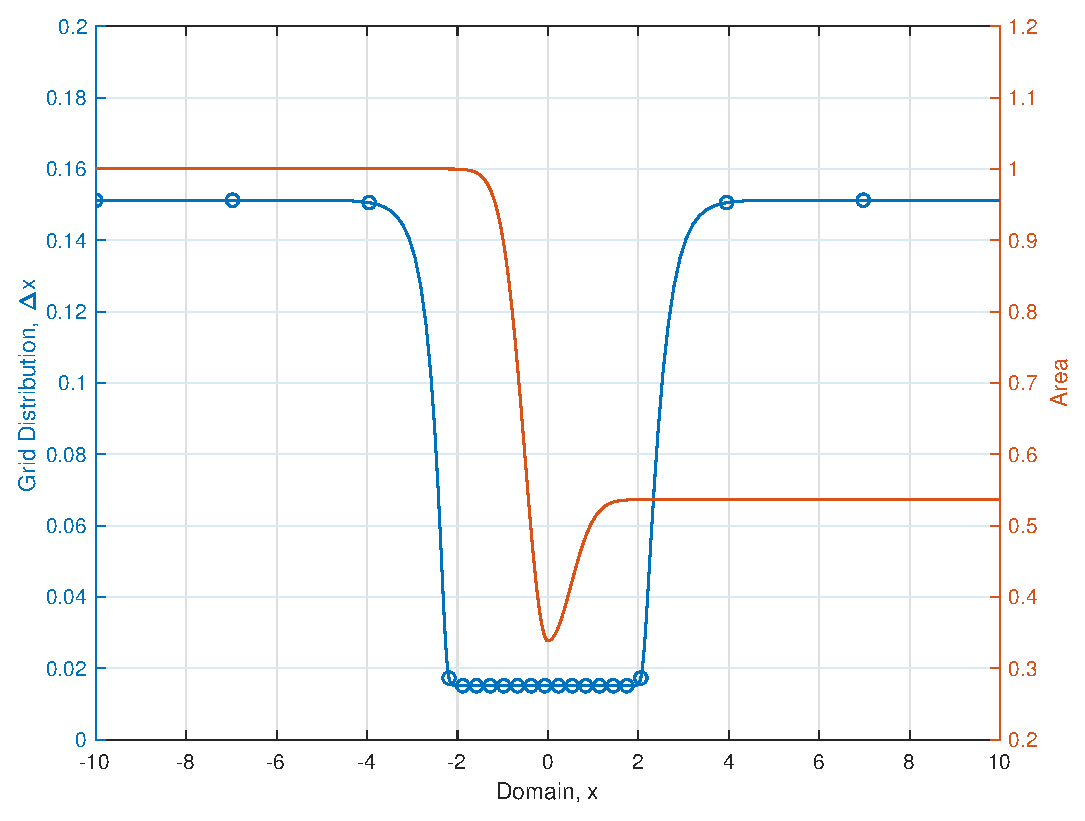
\includegraphics[width=1.0\textwidth]{Figures/Area_dX}
%            \caption{Domain vs Area and Grid Spacing}
            \label{fig:Euler_CD_Area}
        \end{figure}
    \end{columns}
\end{frame}

\begin{frame}{Category 1 Problem 1, Steady State Results}
    \begin{columns}
    \column{1.0\textwidth}
    \begin{itemize}
            \item The mean flow is set as:
\begin{equation*}
	\left\{
	\begin{matrix}
		\overline{\rho} \\
		\overline{u} \\
		\overline{p}
	\end{matrix}
	\right\}~=~
	\left\{
	\begin{matrix}
		1.0 \\
		0.4 \\
		\frac{1}{\gamma}
	\end{matrix}
	\right\}
\end{equation*}
	\end{itemize}
	
\begin{figure}
  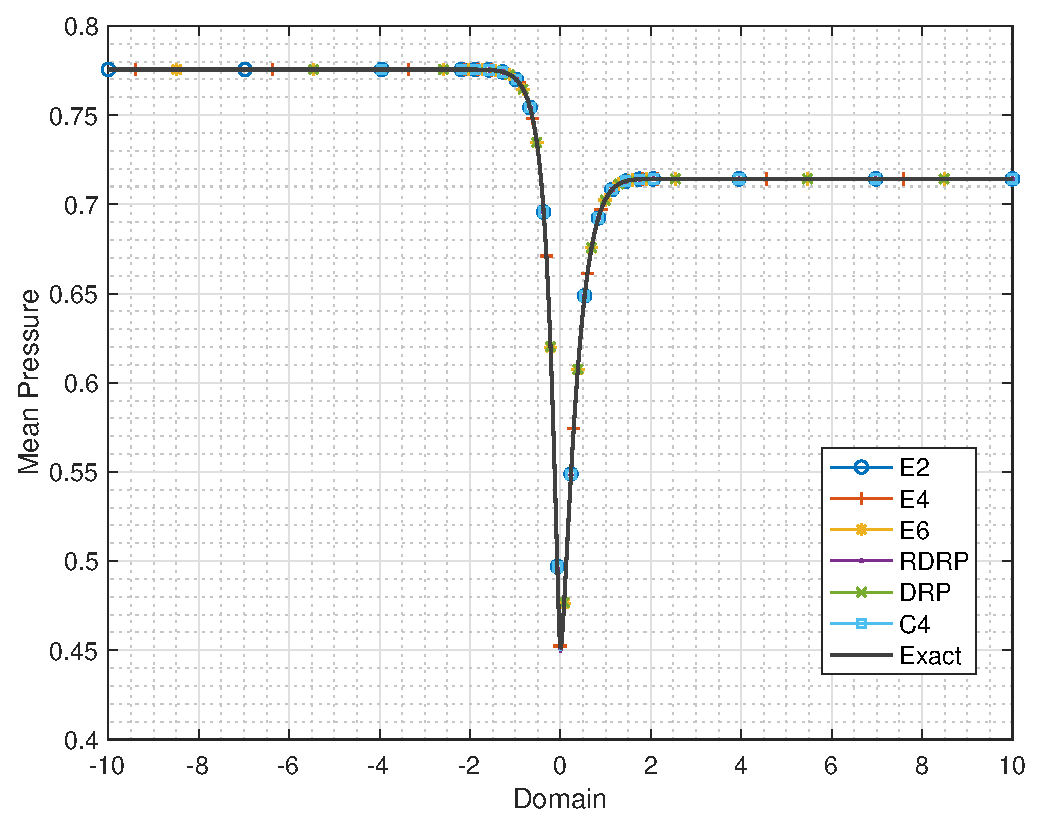
\includegraphics[width=0.48\linewidth]{Figures/C1P1_SteadyState}%
  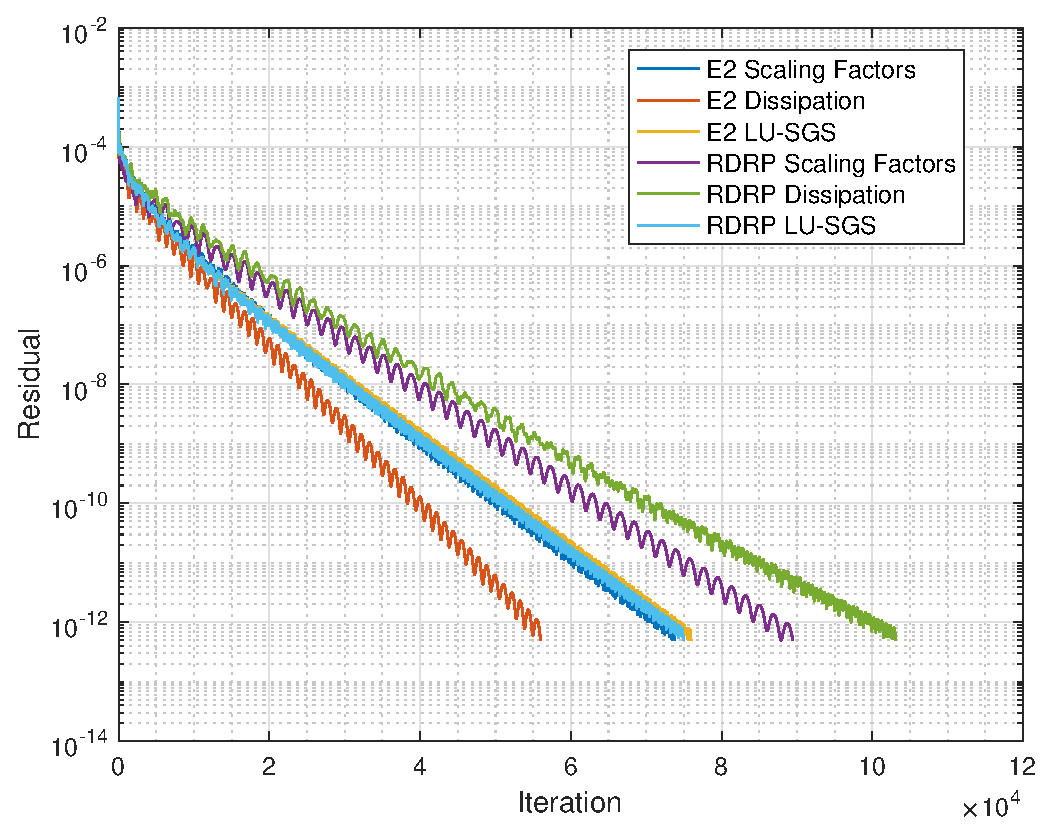
\includegraphics[width=0.48\linewidth]{Figures/C1P1_ROC_E2_vs_RDRP}
\end{figure}

    \end{columns}
\end{frame}

\begin{frame}{Category 1 Problem 1, Unsteady Results}
\begin{columns}
    \column{1.0\textwidth}
    % \usepackage{graphicx}
\begin{table}[htp!]
\centering
\caption{CFL Values for Category 1 Problem 1}
\label{tab:C1P1_CFL}
\begin{tabular}{|l|c|c|c|c|c|c|}
\hline
 & \multicolumn{1}{c|}{\textbf{E2}} & \multicolumn{1}{c|}{\textbf{E4}} & \multicolumn{1}{c|}{\textbf{E6}} & \multicolumn{1}{c|}{\textbf{DRP}} & \multicolumn{1}{c|}{\textbf{RDRP}}& \multicolumn{1}{c|}{\textbf{C4}}\\ \hline
\textbf{$\nu_{physical}$} & \textit{12.521} & \textit{17.518} & \textit{19.858} & \textit{20.834} & \textit{20.834} & \textit{22.237}\\ \hline
\end{tabular}
\end{table}
~~ \newline
\begin{figure}[hbtp!]
	\centering
	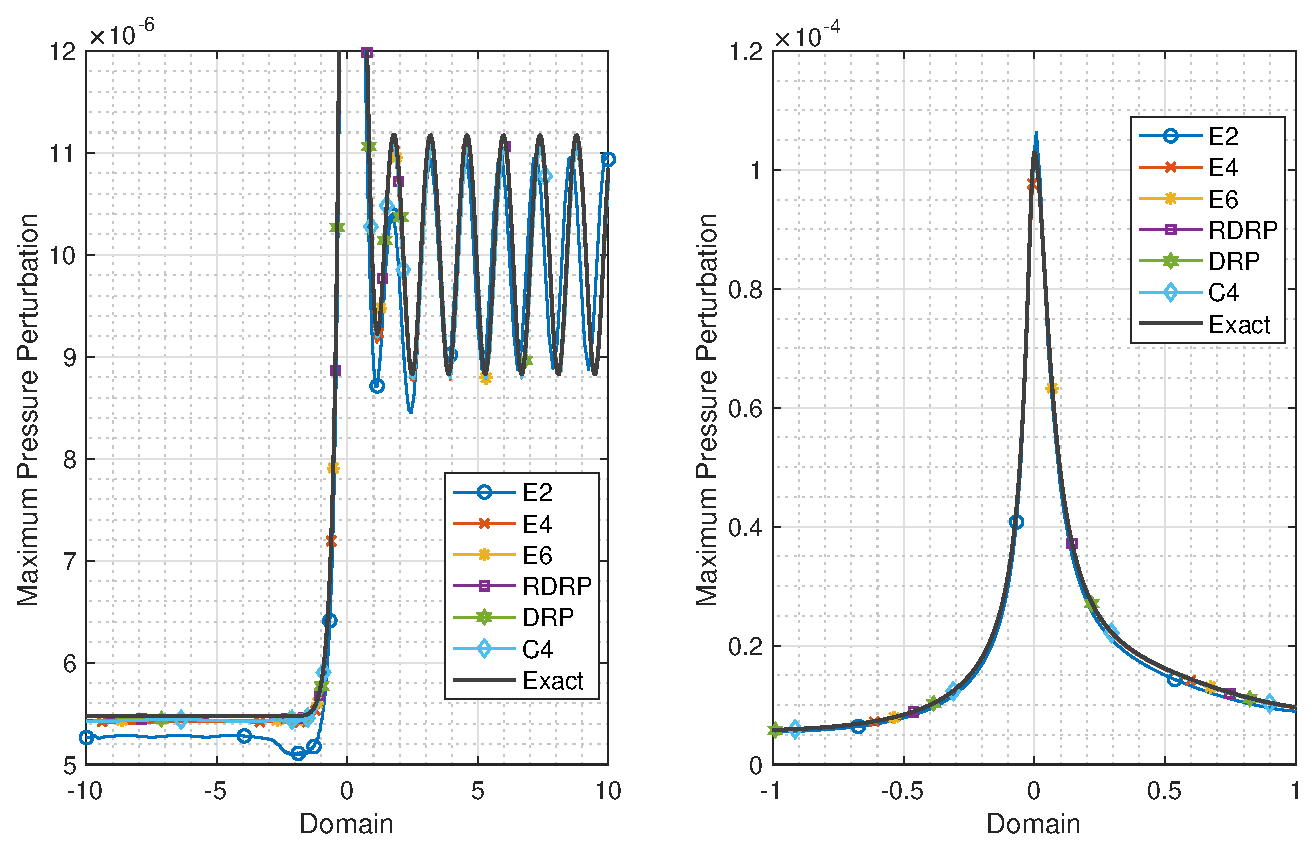
\includegraphics[width=1.0\textheight]{Figures/C1P1_MaxDisturbance_zoom}
	\label{fig:Unsteady_C1P1}
\end{figure}

    \end{columns}
\end{frame}


\section{Conclusions and Future Work}
\begin{frame}{Conclusion}
\begin{columns}
    \column{1.0\textwidth}
        \begin{itemize}
        	\item The present research aimed to establish a highly efficient implicit solver while using higher-order spatial differencing schemes. 
        	\item Through scaling factors, the LHS matrix was replaced with an easier to solve matrix, cutting down on the computational work needed for the iterative steady-state solver. 
        	\item Although the current study is based on one-dimensional problems, the findings suggest stability is possible if scaling factors are used on the LHS spatial difference. 
        	\item The preconditioned matrix was tested against steady and unsteady CAA workshop data; the numerical solution agrees well with the exact.  
        \end{itemize}
    \end{columns}
\end{frame}

\begin{frame}{Acknowledgments}
\begin{columns}
    \column{1.0\textwidth}
        \begin{itemize}
        \item This work is supported by the NASA Advanced Air Transportation Technologies (AATT) Project. 
        \item The authors would like to thank Dr. Edmane Envia of the NASA Glenn Research Center, who is the technical monitor of this work.
        \end{itemize}
        \begin{block}{}
        	Zaid Sabri \\
        	University of Toledo \\
        	Toledo Ohio, 43606 USA \\
        	+1 (567)377-9009 \\
        	zaid.sabri@rockets.utoledo.edu
        \end{block}
    \end{columns}
\end{frame} 
    
\end{document}
